% This file was created with tikzplotlib v0.10.1.
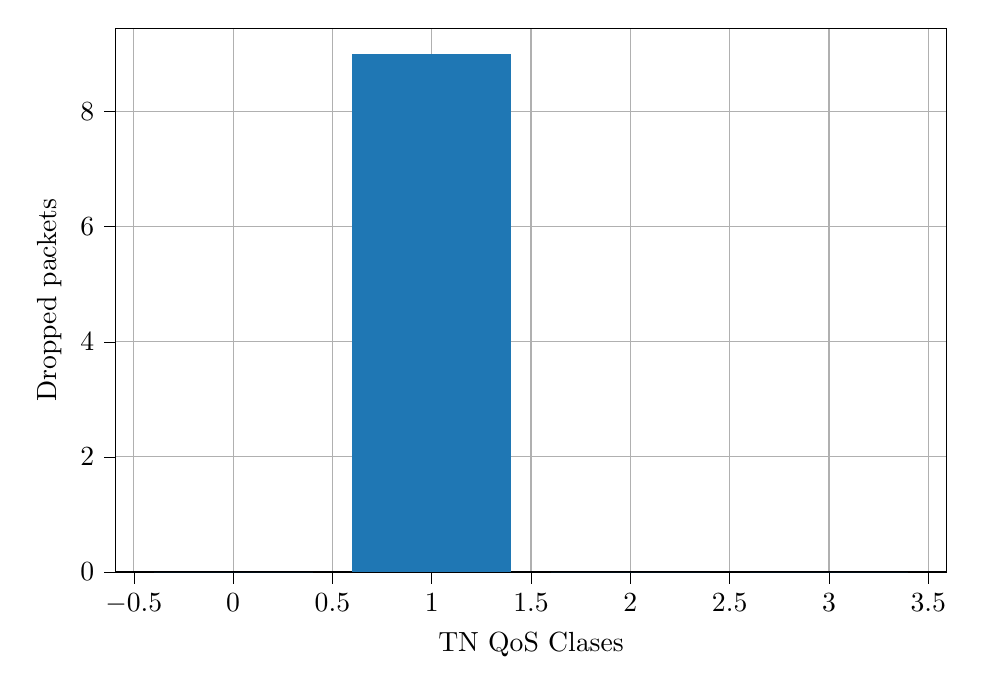
\begin{tikzpicture}

\definecolor{darkgray176}{RGB}{176,176,176}
\definecolor{steelblue31119180}{RGB}{31,119,180}

\begin{axis}[
height=0.7\textwidth,
tick align=outside,
tick pos=left,
width=\textwidth,
x grid style={darkgray176},
xlabel={TN QoS Clases},
xmajorgrids,
xmin=-0.59, xmax=3.59,
xtick style={color=black},
y grid style={darkgray176},
ylabel={Dropped packets},
ymajorgrids,
ymin=0, ymax=9.45,
ytick style={color=black}
]
\draw[draw=none,fill=steelblue31119180] (axis cs:-0.4,0) rectangle (axis cs:0.4,0);
\draw[draw=none,fill=steelblue31119180] (axis cs:0.6,0) rectangle (axis cs:1.4,9);
\draw[draw=none,fill=steelblue31119180] (axis cs:1.6,0) rectangle (axis cs:2.4,0);
\draw[draw=none,fill=steelblue31119180] (axis cs:2.6,0) rectangle (axis cs:3.4,0);
\end{axis}

\end{tikzpicture}
